\begin{figure}[H]
    \centering
    \begin{subfigure}{0.32\textwidth}
        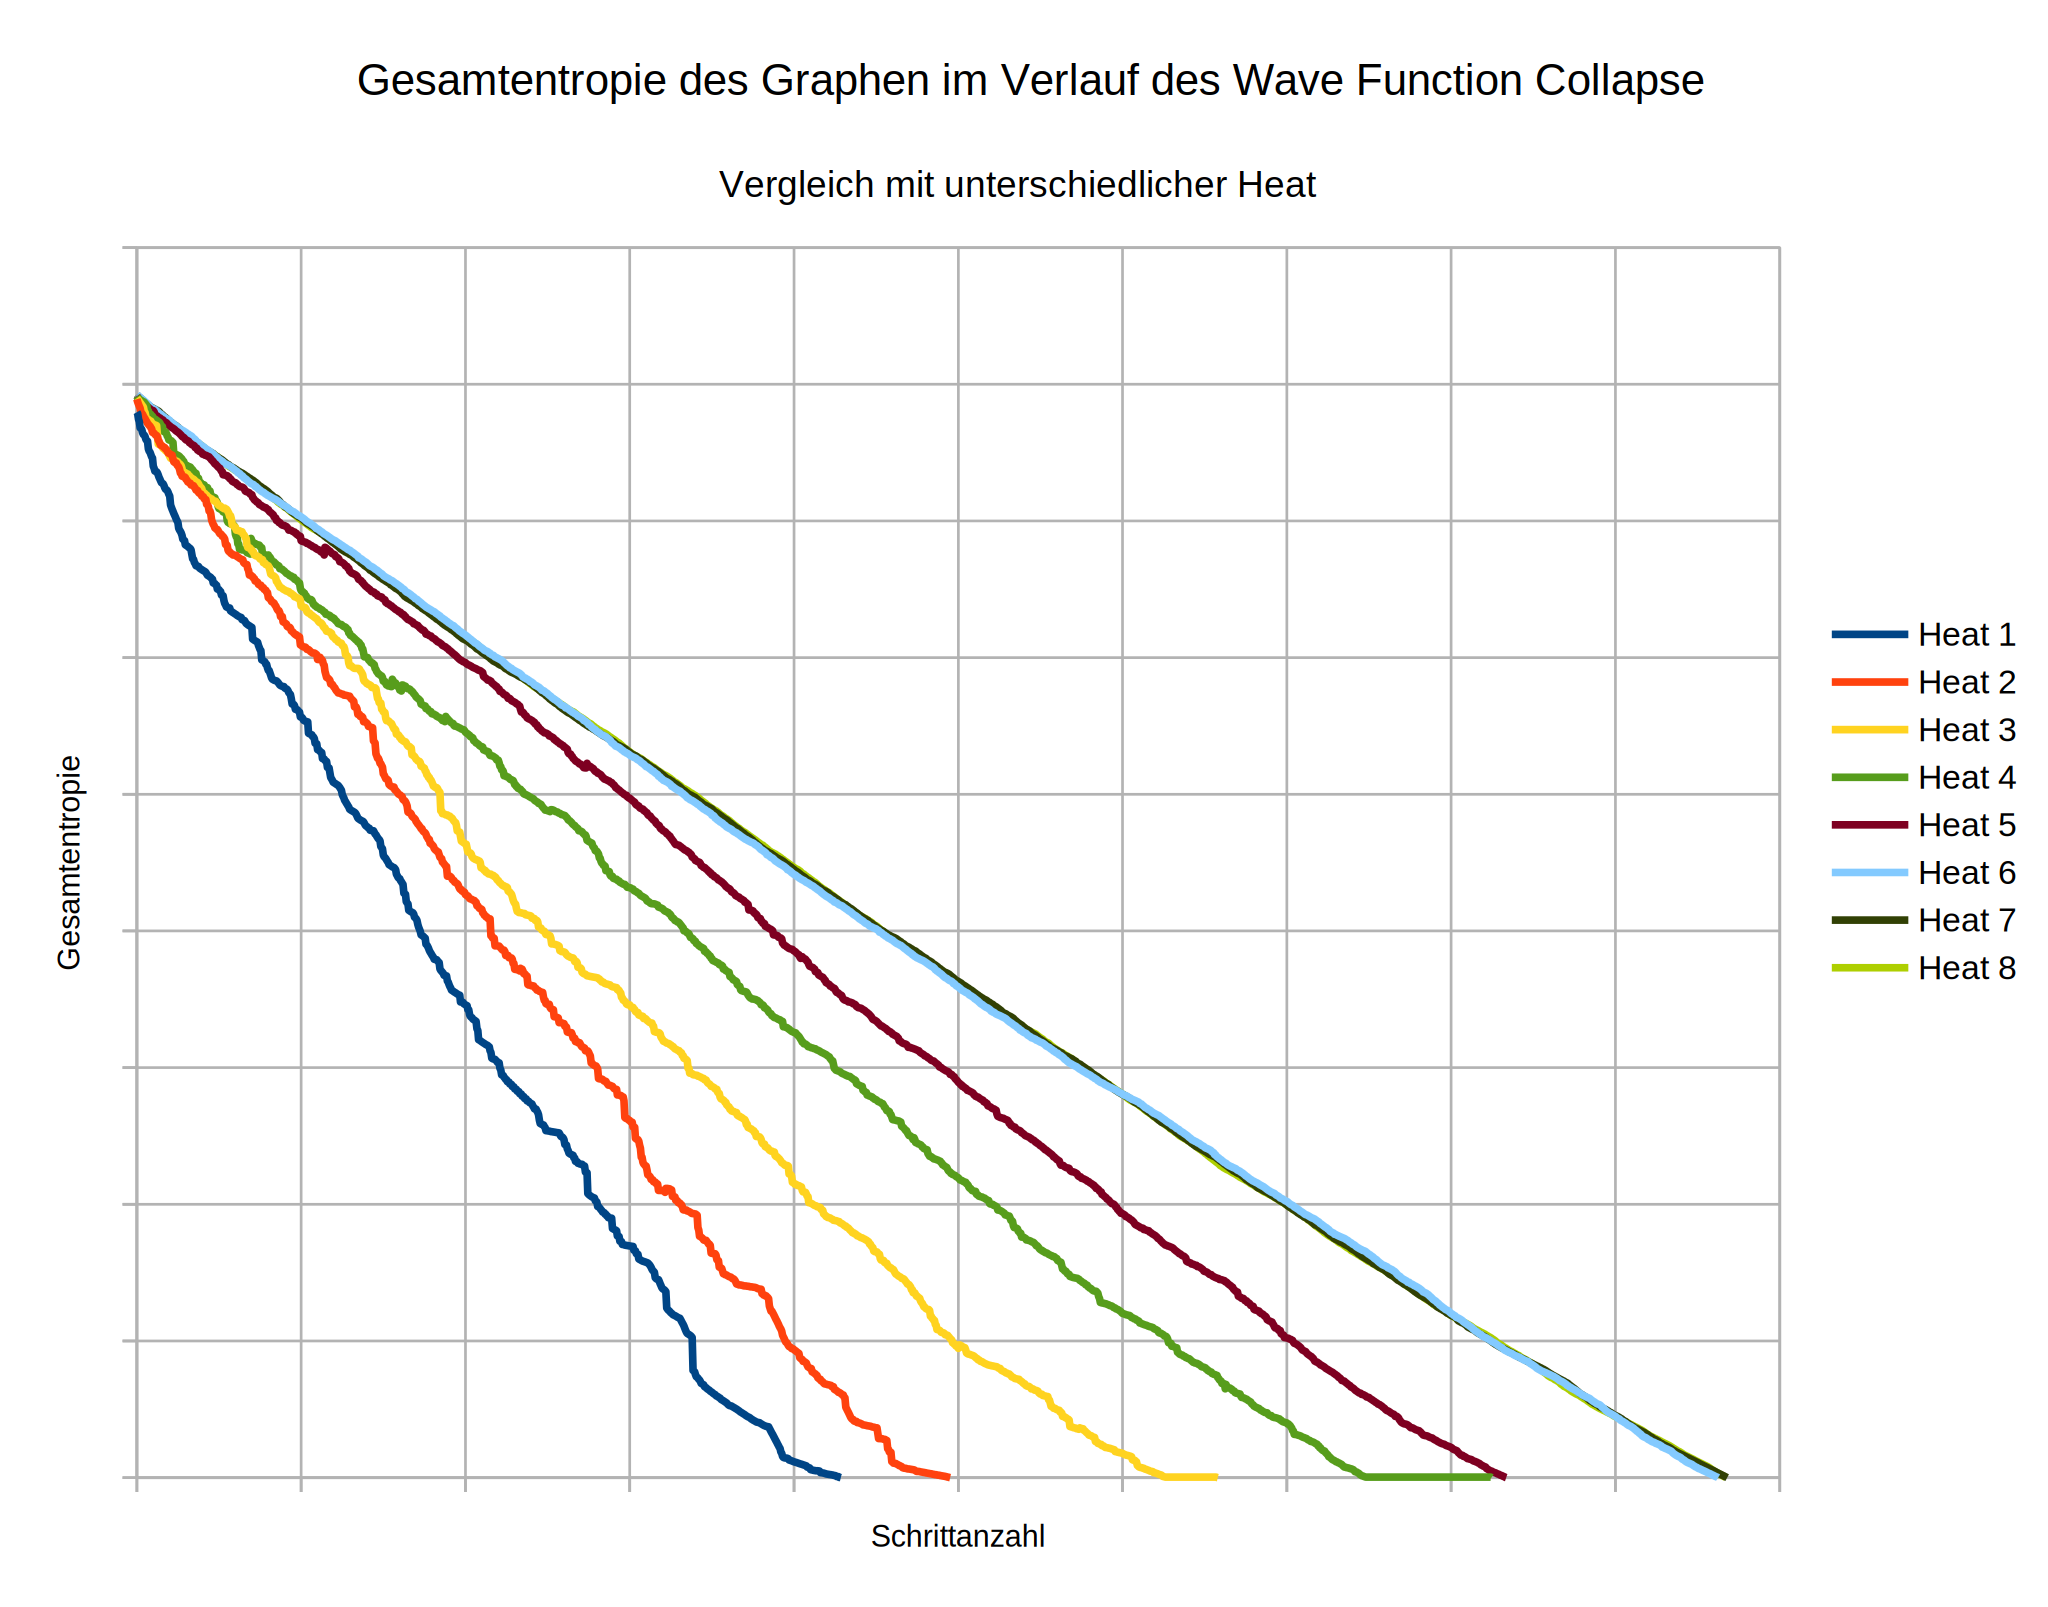
\includegraphics[width=\linewidth]{data/voronoi_clipping/1.png} \caption{}
    \end{subfigure}\hfill
    \begin{subfigure}{0.32\textwidth}
        \includegraphics[width=\linewidth]{data/voronoi_clipping/2.png} \caption{}
    \end{subfigure}\hfill
    \begin{subfigure}{0.32\textwidth}
        \includegraphics[width=\linewidth]{data/voronoi_clipping/3.png} \caption{}
    \end{subfigure}
    
    \vspace{4mm}
    
    \begin{subfigure}{0.32\textwidth}
        \includegraphics[width=\linewidth]{data/voronoi_clipping/4.png} \caption{}
    \end{subfigure}\hfill
    \begin{subfigure}{0.32\textwidth}
        \includegraphics[width=\linewidth]{data/voronoi_clipping/5.png} \caption{}
    \end{subfigure}\hfill
    \begin{subfigure}{0.32\textwidth}
        \includegraphics[width=\linewidth]{data/voronoi_clipping/6.png} \caption{}
    \end{subfigure}
    
    \caption{
        Voronoi-Zellen auf gewünschten Bereich zuschneiden.
        (a) Die Voronoi-Zelle ragt über den Bereich hinaus.
        (b) Ersetze den Eckpunkt außerhalb des Bereichs mit den Schnittpunkt der Kante zum Bereichsrand.
        (c) Der nächste Schnittpunkt mit der linken Seite des Bereichs liegt außerhalb.
        (d) Finde einen besseren Schnittpunkt entlang des anderen Rands.
        (e) Der nächste Schnittpunkt liegt auf dem Eckpunkt der Kante und entfällt.
        (f) Nach zuschneiden der letzten Kante erhalten wir eine korrigierte Voronoi-Zelle.
    }
    \label{fig:voronoi_clipping}
\end{figure}